\subsection{Zigbee2MQTT}
Um das offizielle Zigbee2MQTT Home Assistant Add-on nutzen zu können, müssen wir zunächst im Supervisor Add-on Shop (vgl. Abb. \ref{fig:ha14}: \nameref{fig:ha14}) das Repository\footnote{GITHUB: \url{https://github.com/zigbee2mqtt/hassio-zigbee2mqtt}} hinzufügen. 
Hierdurch erhalten wir die Möglichkeit, das Add-on auf unserem Home Assistant zu installieren. 
Nachdem das geschehen ist, können wir das Add-on Zigbee2MQTT installieren (vgl. Abb. \ref{fig:ha16}: \nameref{fig:ha16}). 
An diesem Punkt bietet sich uns die Möglichkeit, die Zigbee2MQTT ,,configuration.yaml'' einzusehen (vgl. Abb. \ref{fig:ha18}: \nameref{fig:ha18} und Anhang \ref{ah_yaml_ha_configuration}: \nameref{ah_yaml_ha_configuration}).\\
\noindent Hier ist darauf zu achten, dass der Parameter von ,,permit-join'' lediglich für das Einlernen von neuen Zigbee-Geräten auf ,,true'' gesetzt wird.
Um einen sauberen ersten Start von Zigbee2MQTT gewährleisten zu können, muss nun noch der ,,Serial Port'' des Zigbee Adapters überprüft werden. 
Zu diesem Zweck navigieren wir über ,,Supervisor'' (vgl. Abb. \ref{fig:ha19}: \nameref{fig:ha19}) zu ,,System'' (vgl. Abb. \ref{fig:ha19}: \nameref{fig:ha19}) und dort unter ,,Host'' zu ,,Hardware''. 
In diesem Fenster sehen wir sämtliche Hardware, die mit dem Host-System, also in unserem Fall dem Raspberry Pi, verbunden ist (vgl. Abb. \ref{fig:ha19}: \nameref{fig:ha19}). \\
\noindent Nachdem sicher gestellt ist, dass der ,,Serial Port'' mit dem tatsächlichen Port übereinstimmt, können wir das Add-on starten (vgl. Abb. \ref{fig:ha17}: \nameref{fig:ha17}). \\
\noindent Das Einlernen von neuen Leuchtmitteln und Geräten gestaltet sich, sofern die Datei ,,configuration.yaml'' (s. Anhang \ref{ah_yaml_devices}: \nameref{ah_yaml_devices}) beachtet wurde, deutlich einfacher.
Zuerst muss das Leuchtmittel oder Gerät nach Herstellerangabe zurückgesetzt werden. 
Danach wird das Gerät automatisch von Zigbee2MQTT erfasst und eingelernt.
Eingelernte Geräte werden in der Datei ,,devices.yaml'' (vgl. \ref{ah_yaml_devices}: \nameref{ah_yaml_devices}) gespeichert und sind dadurch als Entitäten in Home Assistant steuerbar.
\begin{figure}[H]
    \begin{subfigure}{.5\linewidth}
        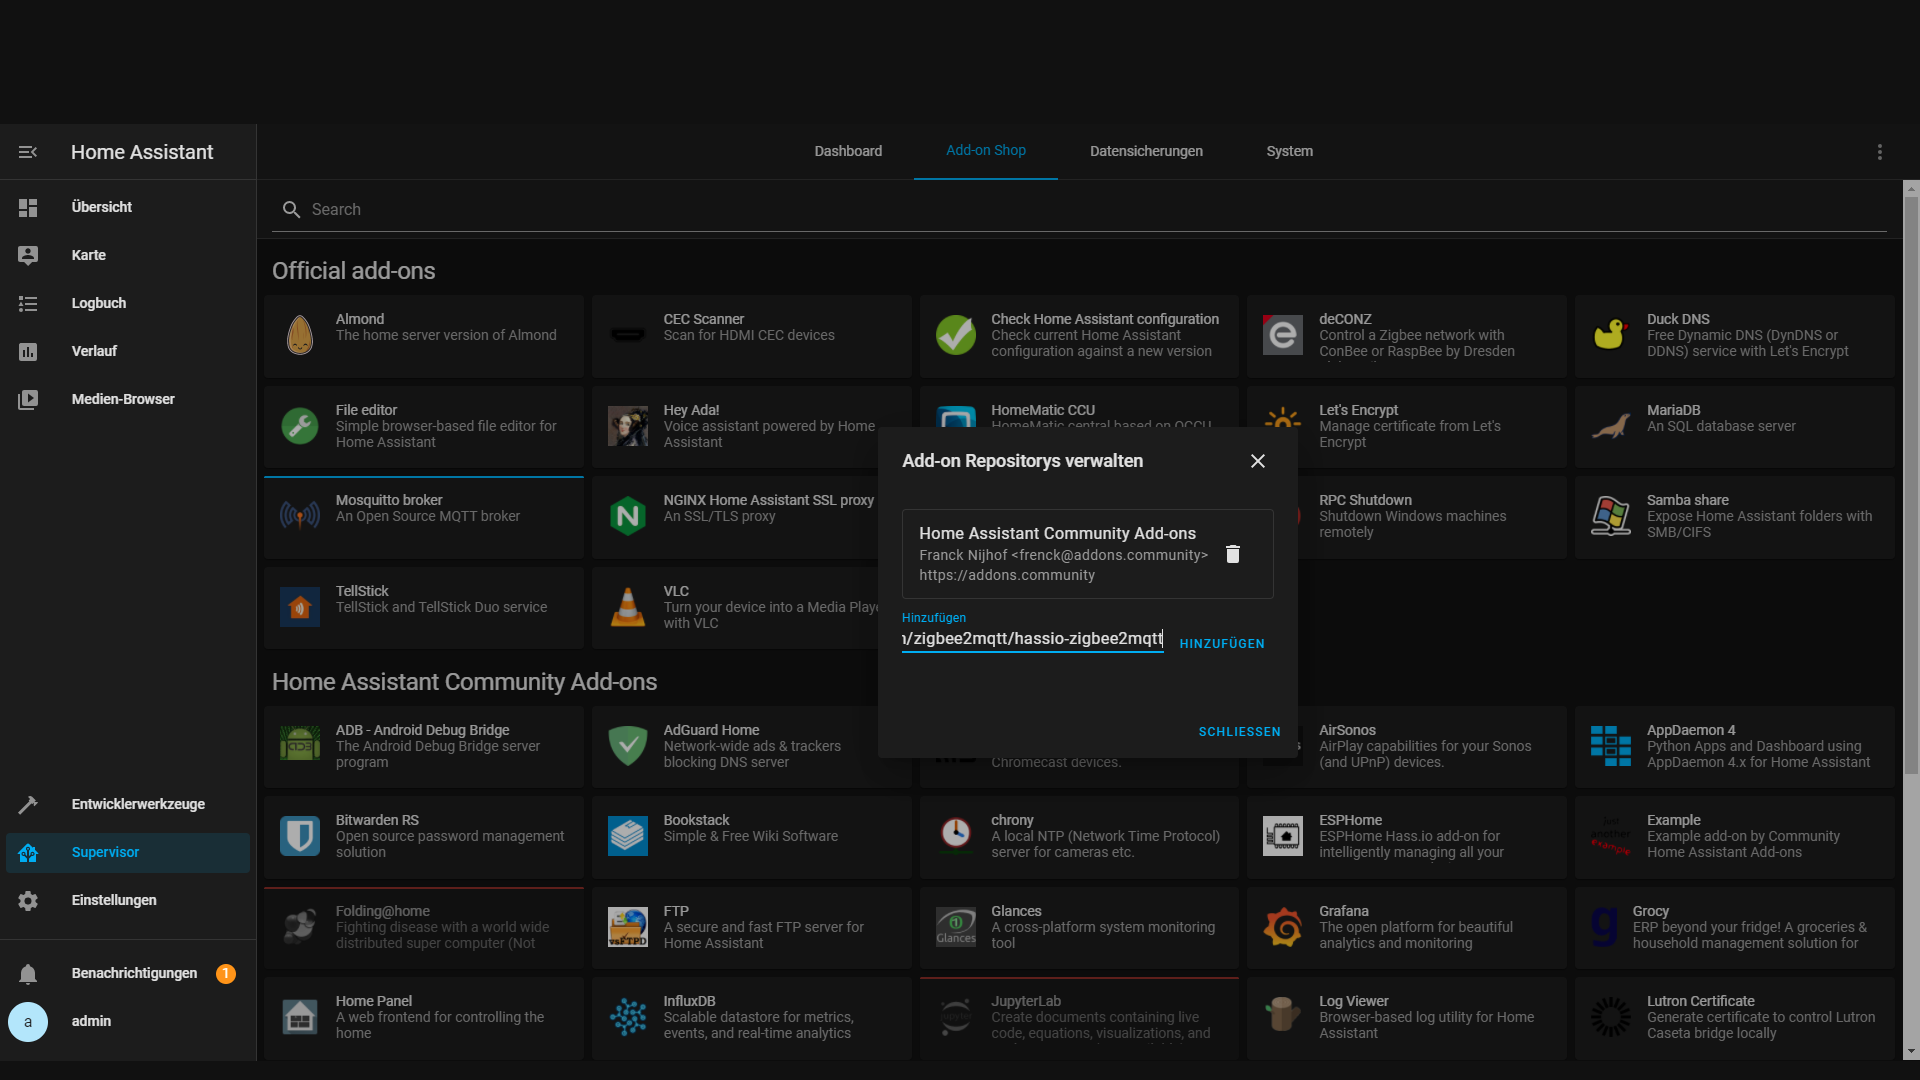
\includegraphics[width=1\textwidth]{img/HA18.png}
        \caption{Repository in Add-on Shop einpflegen}
        \label{fig:ha14}
    \end{subfigure}
%    \begin{subfigure}{.5\linewidth}
%        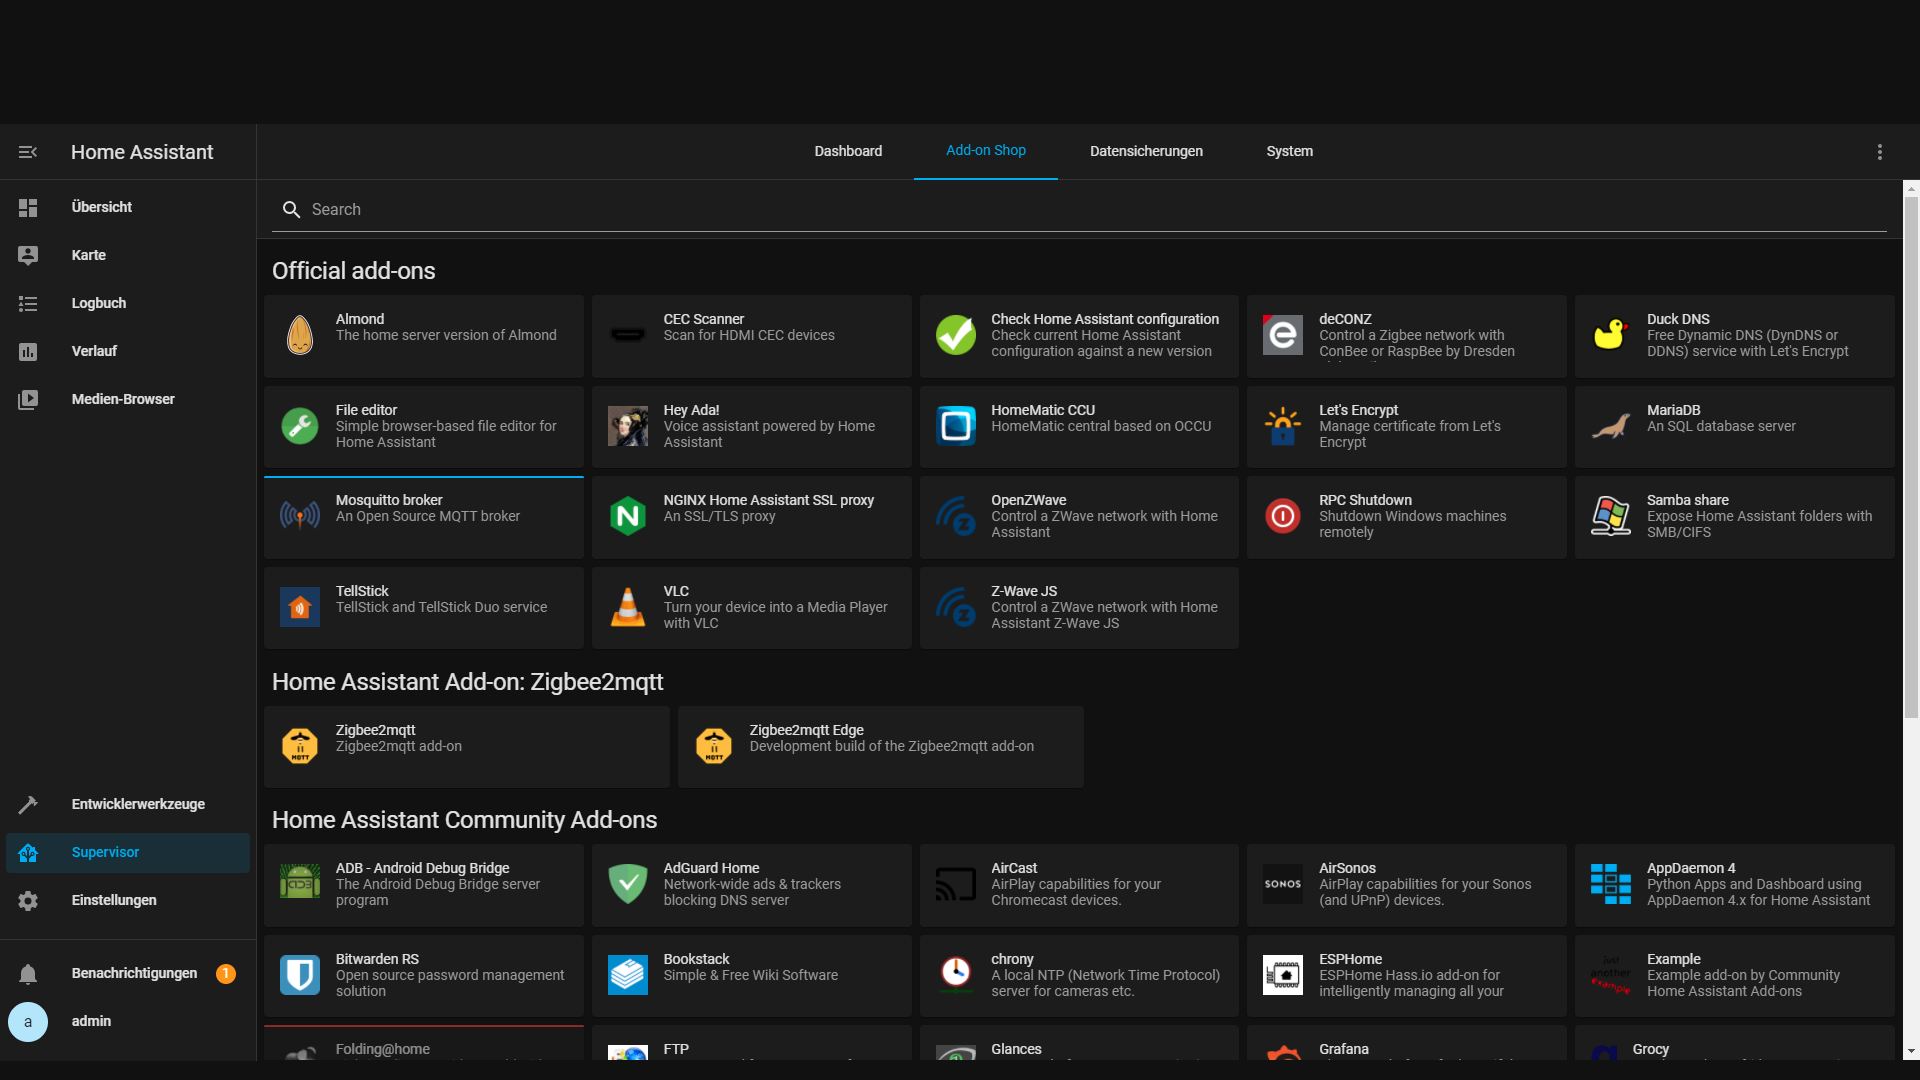
\includegraphics[width=1\textwidth]{img/HA19.png}
%        \caption{Supervisor Add-on Shop}
%        \label{fig:ha15}
%    \end{subfigure}
    \begin{subfigure}{.5\linewidth}
        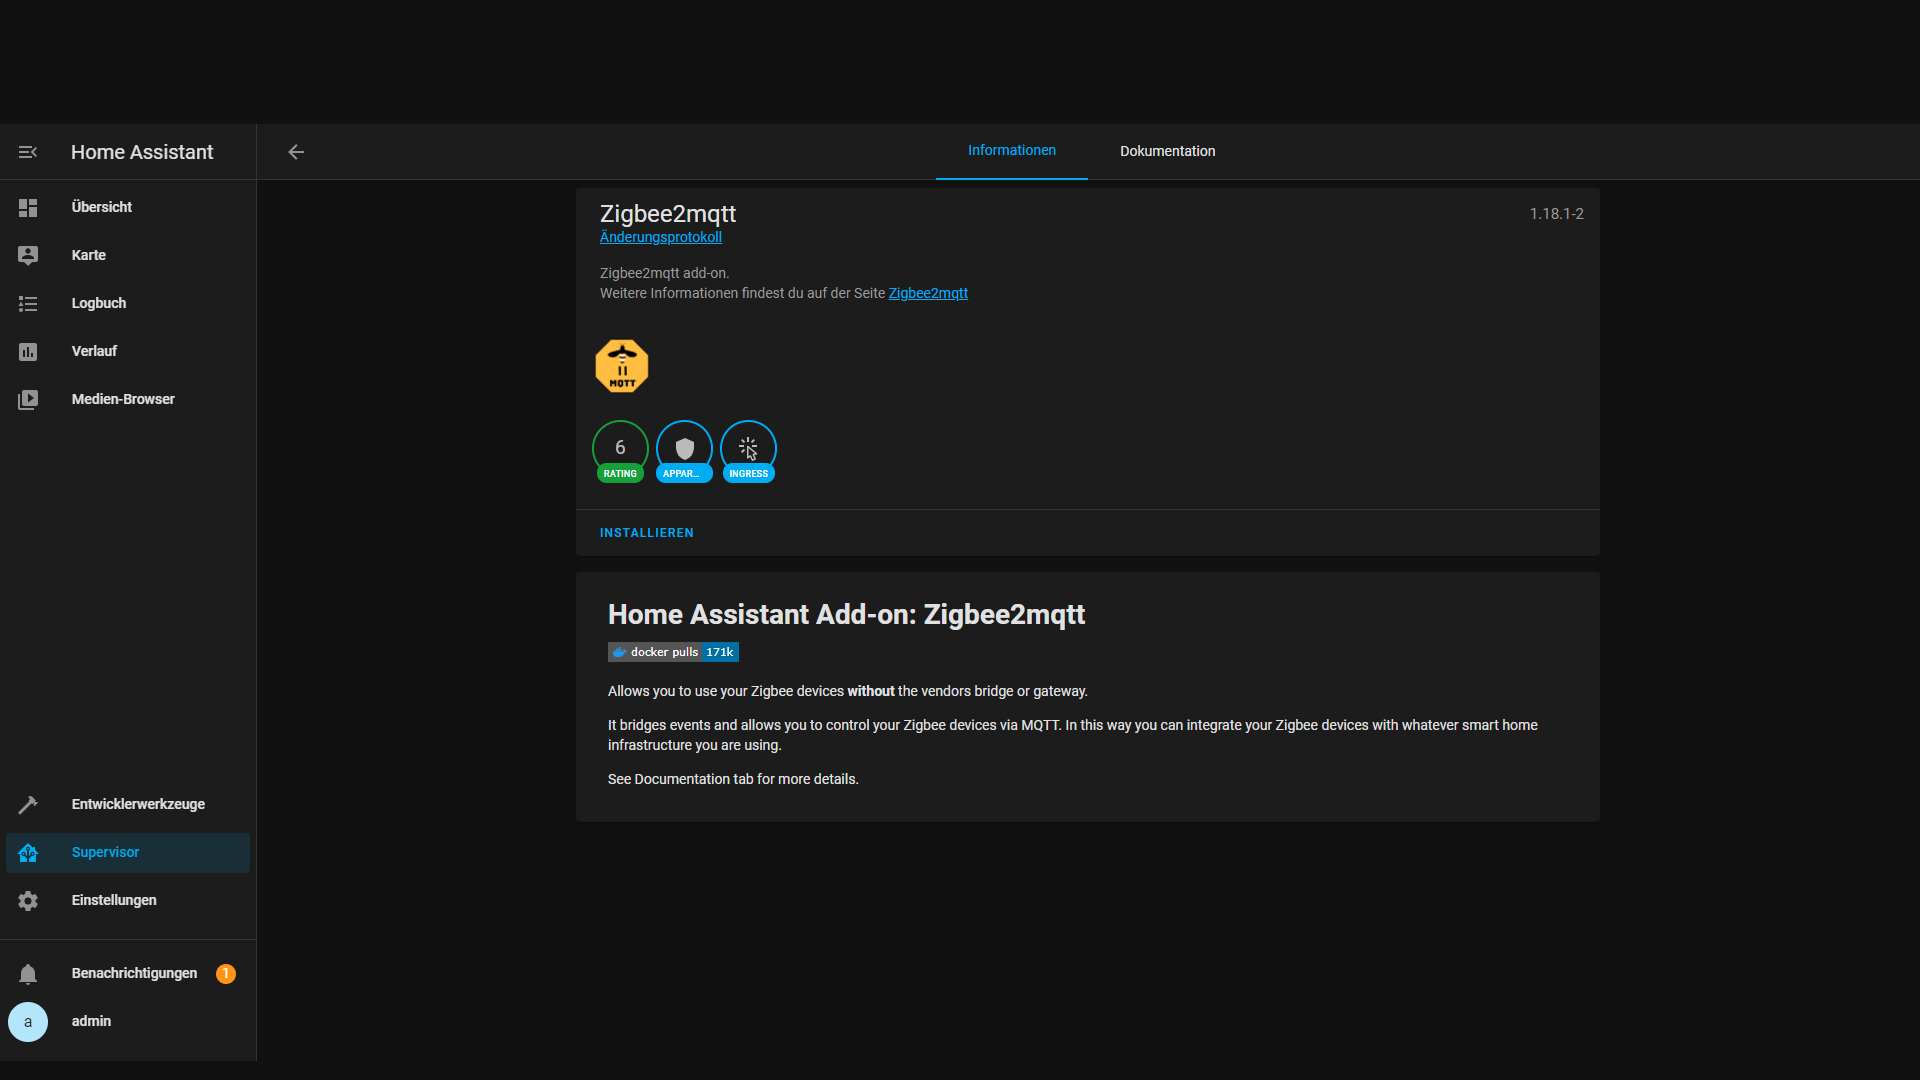
\includegraphics[width=1\textwidth]{img/HA20.png}
        \caption{Zigbee2MQTT Add-on Seite}
        \label{fig:ha16}
    \end{subfigure}
    \begin{subfigure}{.5\linewidth}
        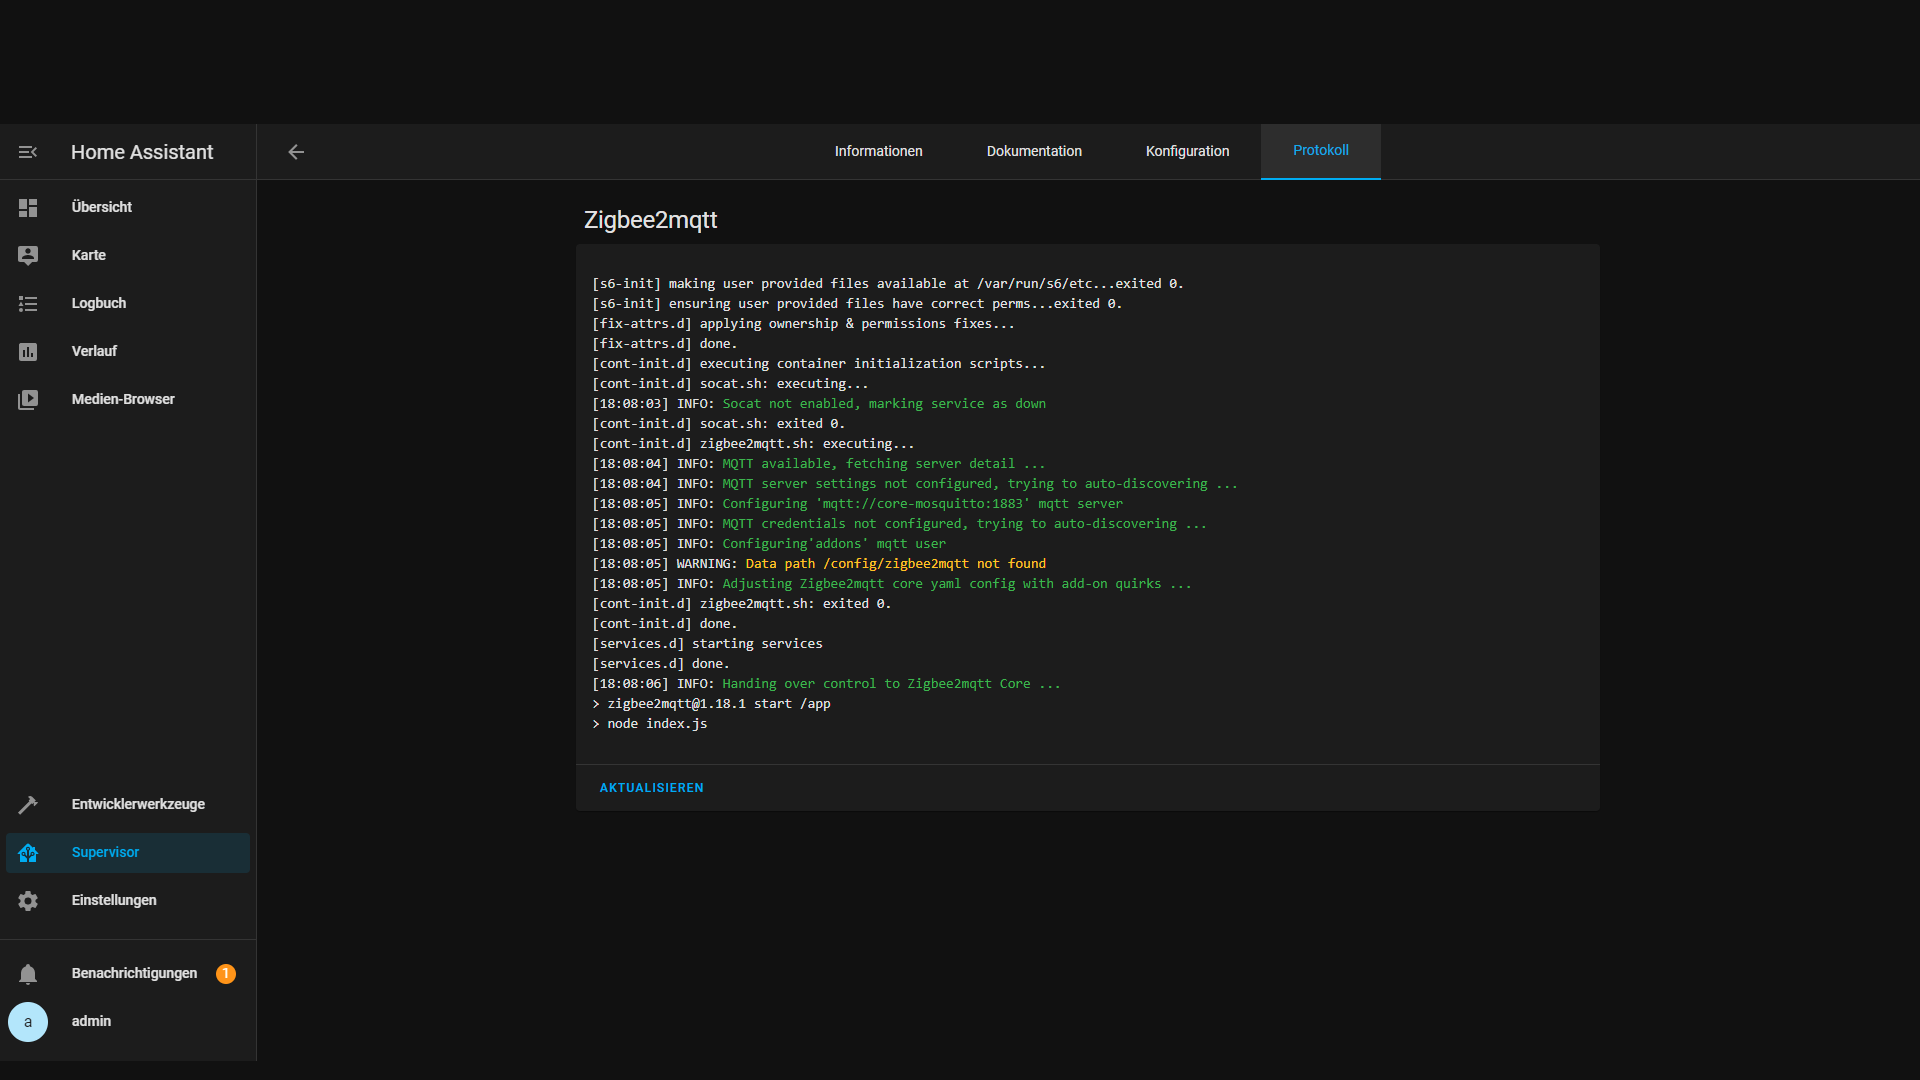
\includegraphics[width=1\textwidth]{img/HA22.png}
        \caption{Configuration.yaml}
        \label{fig:ha18}
    \end{subfigure}
    \begin{subfigure}{.5\linewidth}
        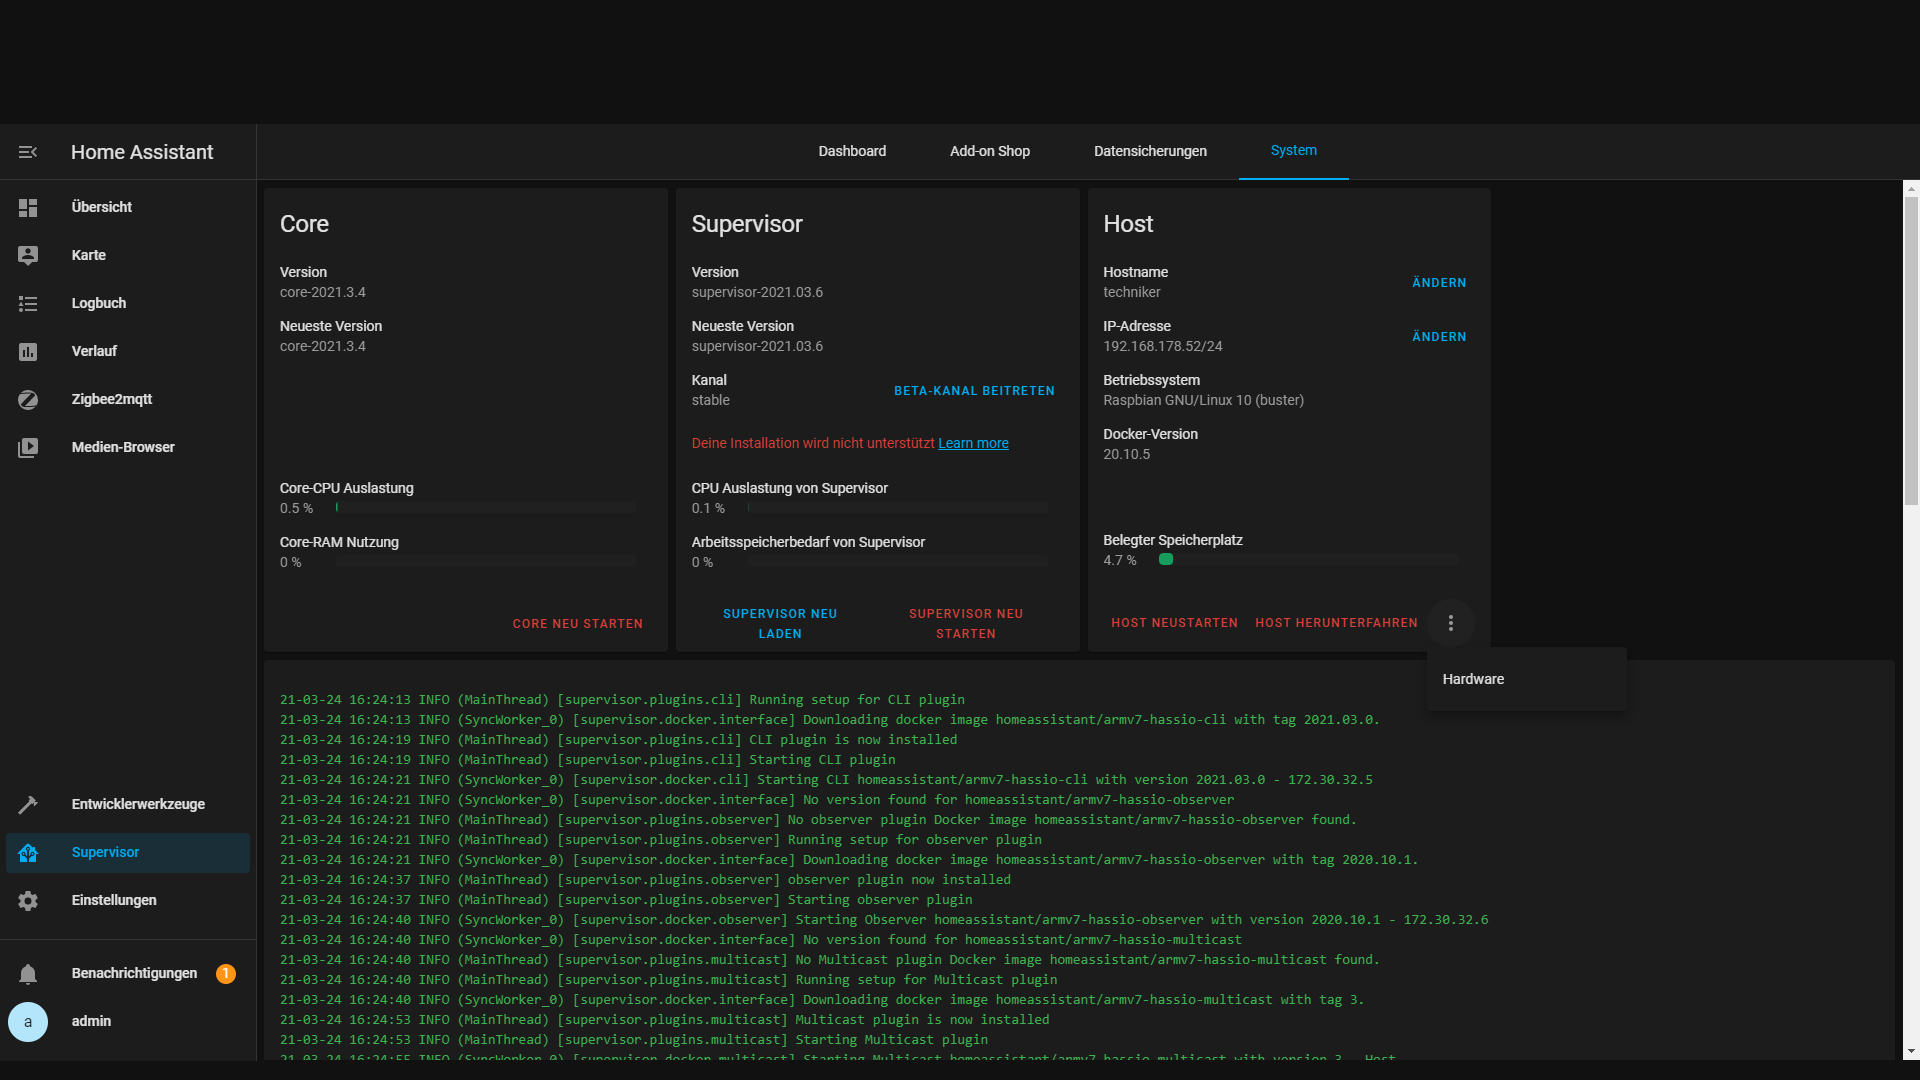
\includegraphics[width=1\textwidth]{img/HA23.png}
        \caption{Supervisor Systeminformationen}
        \label{fig:ha19}
    \end{subfigure}
    \begin{subfigure}{.5\linewidth}
        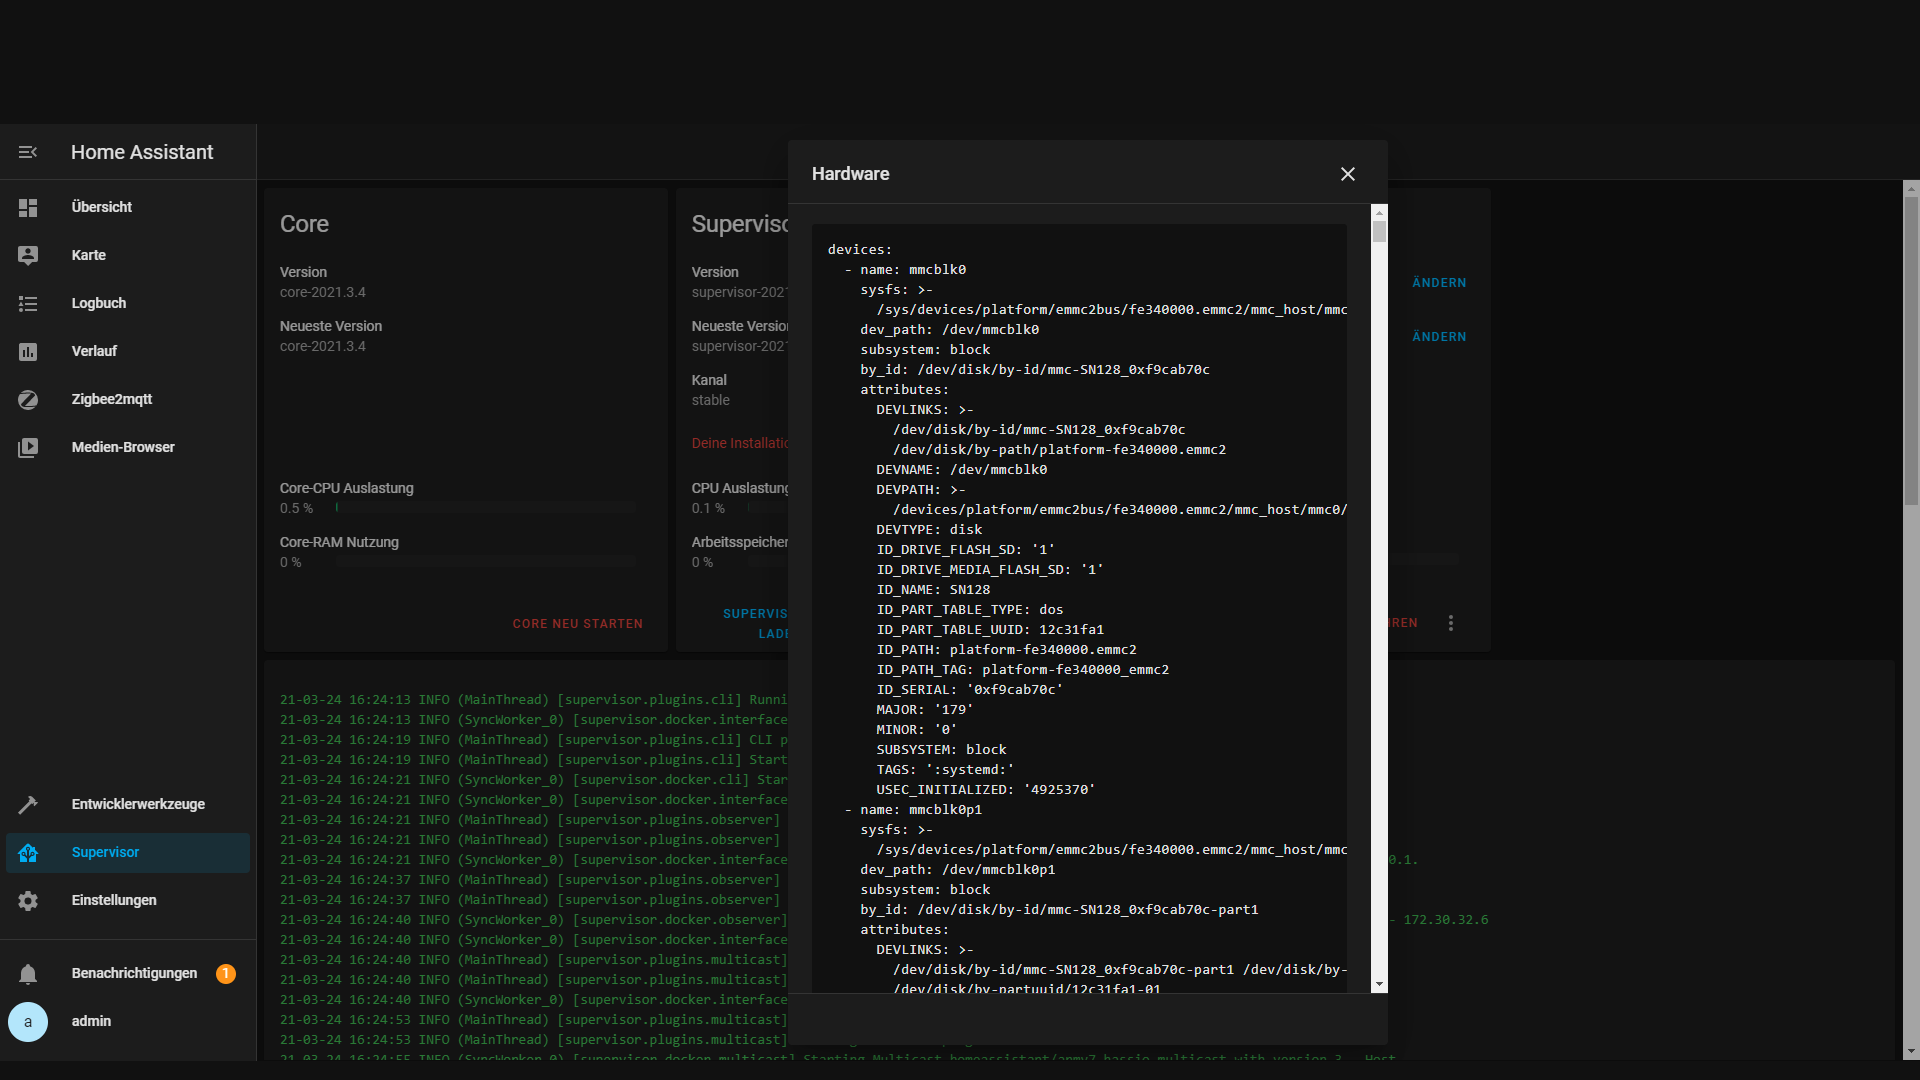
\includegraphics[width=1\textwidth]{img/HA24.png}
        \caption{Auflistung der Hardware}
        \label{fig:ha20}
    \end{subfigure}
    \begin{subfigure}{.5\linewidth}
        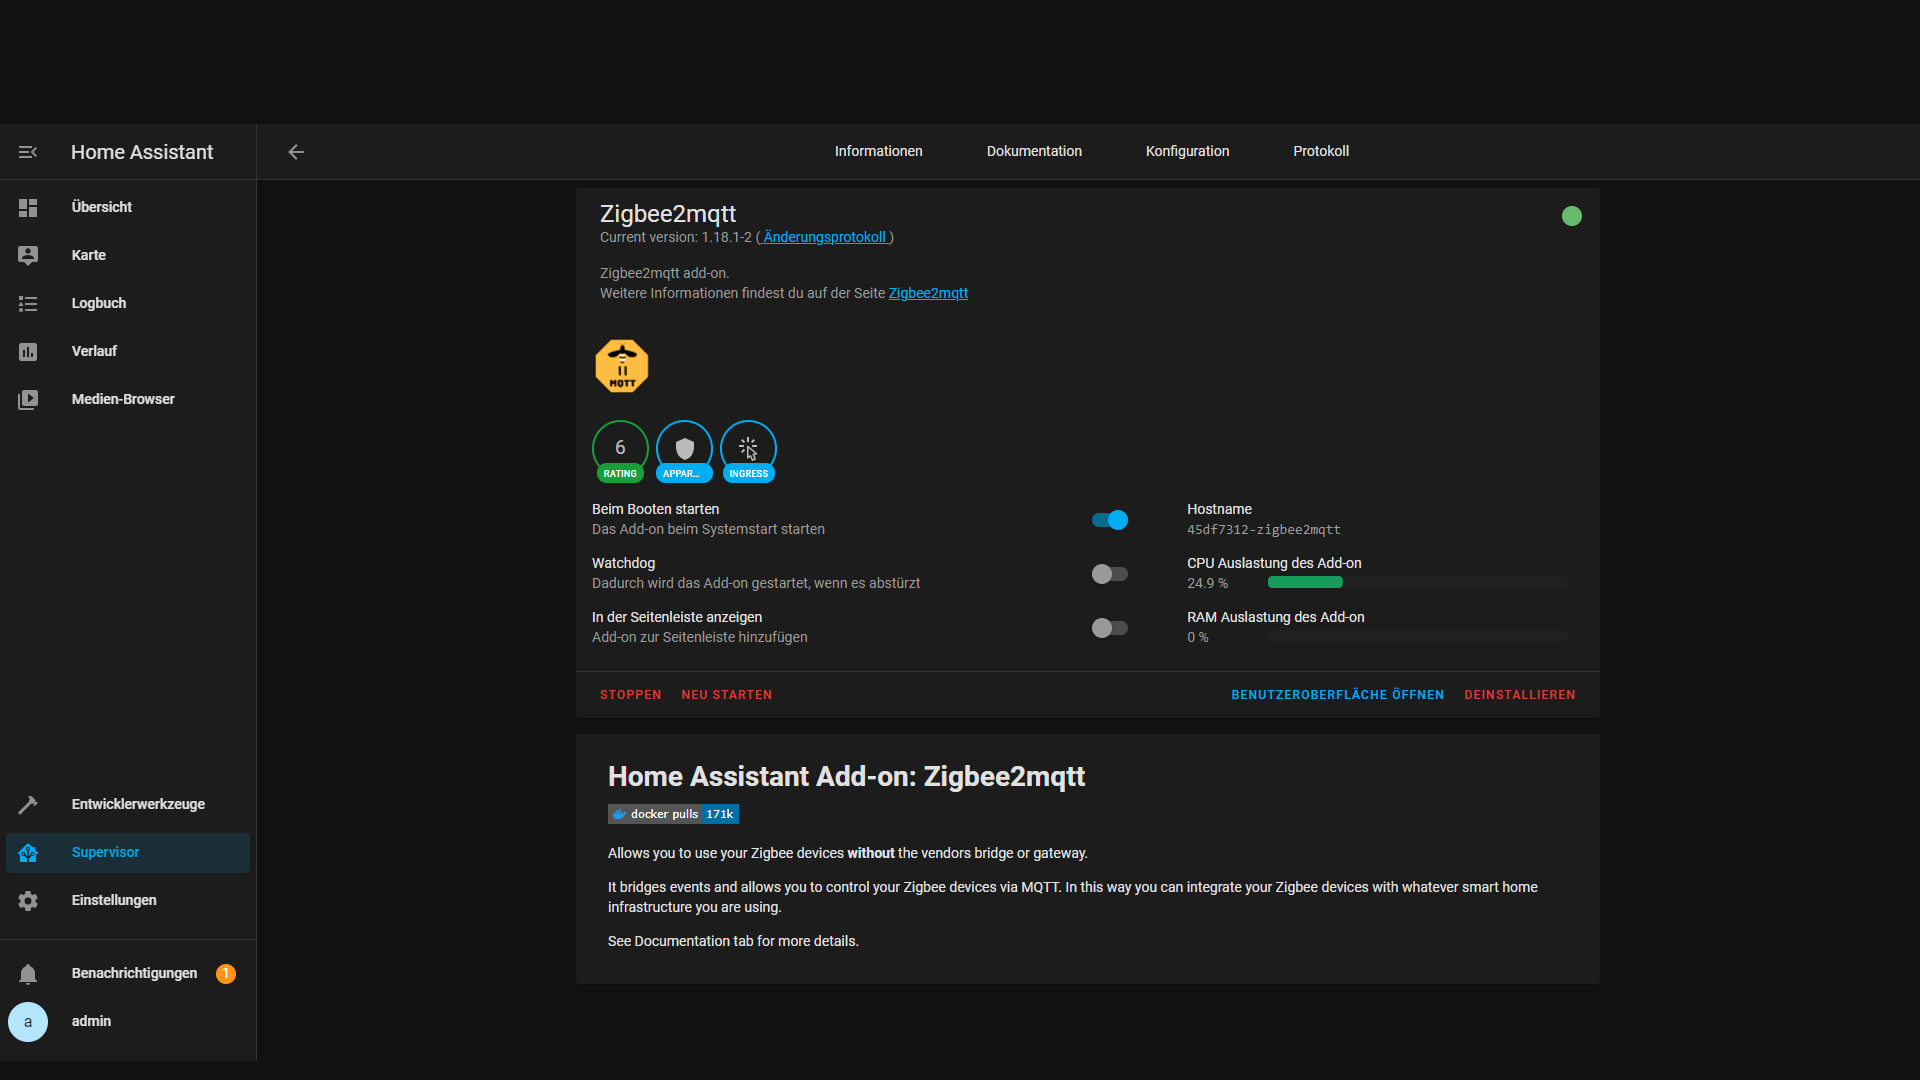
\includegraphics[width=1\textwidth]{img/HA21.png}
        \caption{Aktiviertes Zigbee2MQTT Add-on}
        \label{fig:ha17}
    \end{subfigure}
\end{figure}

